\documentclass[a4paper,twoside,zihao=5,UTF8]{ctexrep}

\ctexset{
	section = {
		format+ = \zihao{-4} \heiti \raggedright,
		name = {,、},
		number = \chinese{section},
		beforeskip = 1.0ex plus 0.2ex minus .2ex,
		afterskip = 1.0ex plus 0.2ex minus .2ex,
		aftername = \hspace{0pt}
	},
	subsection = {
		format+ = \zihao{5} \heiti \raggedright,
		name = {\thesubsection、},
		name = {,、},
		number = \arabic{subsection},
		beforeskip = 1.0ex plus 0.2ex minus .2ex,
		afterskip = 1.0ex plus 0.2ex minus .2ex,
		aftername = \hspace{0pt}
	}
}

\usepackage{titling}

\usepackage[utf8]{inputenc}
\usepackage[T1]{fontenc}

\usepackage{lmodern}
\usepackage{microtype}
\usepackage{blindtext}


\usepackage{listings}
\usepackage{xcolor}

\usepackage{geometry}
\geometry{left=2.3cm,right=2cm,top=2.5cm,bottom=2.0cm}

\usepackage{amsmath}
\usepackage{float}
\usepackage{hyperref}

\usepackage{graphics}
\usepackage{graphicx}

\usepackage{subfigure}
\usepackage{epsfig}
\usepackage{float}

\usepackage{algorithm}
\usepackage[noend]{algpseudocode}

\usepackage{booktabs}
\usepackage{threeparttable}
\usepackage{longtable}
\usepackage{listings}

% cite package, to clean up citations in the main text. Do not remove.
\usepackage{cite}

\usepackage{color,xcolor}

%% The amssymb package provides various useful mathematical symbols
\usepackage{amssymb}
%% The amsthm package provides extended theorem environments
\usepackage{amsthm}
\usepackage{amsfonts}
\usepackage{enumerate}
\usepackage{enumitem}
\usepackage{listings}

\usepackage{indentfirst}
\usepackage{setspace}
\usepackage{siunitx}

\newcommand{\subtitle}[1]{%
  \posttitle{%
    \par\end{center}
    \begin{center}\large#1\end{center}
    \vskip0.5em}%
}

%%%%%%%%%%%%%
\newcommand{\Authors}{熊恪峥 \ 徐昊 \ 陈奕凝}  % Replace your name here
\newcommand{\BookTitle}{Transformer框架下的的遥感图象分割}  % Change your paper title here
\newcommand{\BookSubtitle}{基于ST-UNet} % Replace the type of your report here
\newcommand{\Date}{2022年5月4日}
%%%%%%%%%%%%%

%% Page header and footer setting
\usepackage{fancyhdr}
\usepackage{lastpage}
\pagestyle{fancy}
\fancyhf{}
% This requires the document to be twoside
\fancyhead[L]{\texttt{\Authors }}
\fancyhead[CE]{\texttt{\BookTitle }}
\fancyhead[CO]{\leftmark }
\fancyhead[R]{\texttt{第{\thepage}页,共\pageref*{LastPage}页}}

\graphicspath{ {images/} }


\frenchspacing

\title{\BookTitle}
\subtitle{\BookSubtitle}
\author{\Authors}
\date{\Date}


\begin{document}

\maketitle
\thispagestyle{empty}

\tableofcontents 
\thispagestyle{empty}

\clearpage
\setcounter{page}{1}

\part{选题}
\chapter{题目概述}
本队选题是“遥感地块影像分割”,赛题旨在对遥感影像进行像素级内容解析,并对遥感影像中感兴趣的类别进行提取和分类,
以衡量遥感影像地块分割模型在多个类别(如建筑、道路、林地等)上的效果。数据集为多个地区已脱敏的遥感影像数据,
包含$66,653$张分辨率为$2\mathop{m}/\mathop{pixel}$,尺寸为$256 \times 256$的PNG图片

\begin{figure}[htbp]
    \centering
	\caption{数据集示例}
	\label{fig:trainsetexample}
	
	\subfigure[训练集]{
		\begin{minipage}[t]{0.28\linewidth}
			\centering
			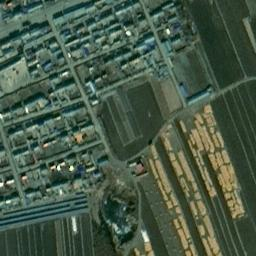
\includegraphics[width=\textwidth]{example/e1c.jpg}
	\end{minipage}}
	\subfigure[标注]{
		\begin{minipage}[t]{0.28\linewidth}
			\centering
			
\includegraphics[width=\textwidth]{example/e1bw.png}
	\end{minipage}}

    \subfigure[训练集]{
		\begin{minipage}[t]{0.28\linewidth}
			\centering
			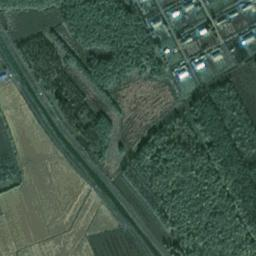
\includegraphics[width=\textwidth]{example/e2c.jpg}
	\end{minipage}}
	\subfigure[标注]{
		\begin{minipage}[t]{0.28\linewidth}
			\centering
			
\includegraphics[width=\textwidth]{example/e2bw.png}
	\end{minipage}}
	
\end{figure}

\part{设计思路}

\chapter{设计概述}
Transfomer是一种在自然语言处理领域中流行的模型。近年来,Transfomer的成功
为涉及全局关系的深度学习领域的研究提供了新的方法。Visual Transfomer (ViT)\cite{vit}将Transfomer
引入计算机视觉领域,获得了良好效果。基于ViT的语义分割\cite{segmenter}在ADE20K数据集上
达到State-of-the-art,超越了其他同类模型。Swin-Transfomer\cite{swin}通过构建
层次化的Transformer改进了ViT,并且引入Locality,在ADE20K数据集上达到了53.5的mIOU。
因此在语义分割任务上,Swin-Transformer是一种极具前景的主干网络,有很好的效果预期。

\begin{figure}[htbp]
    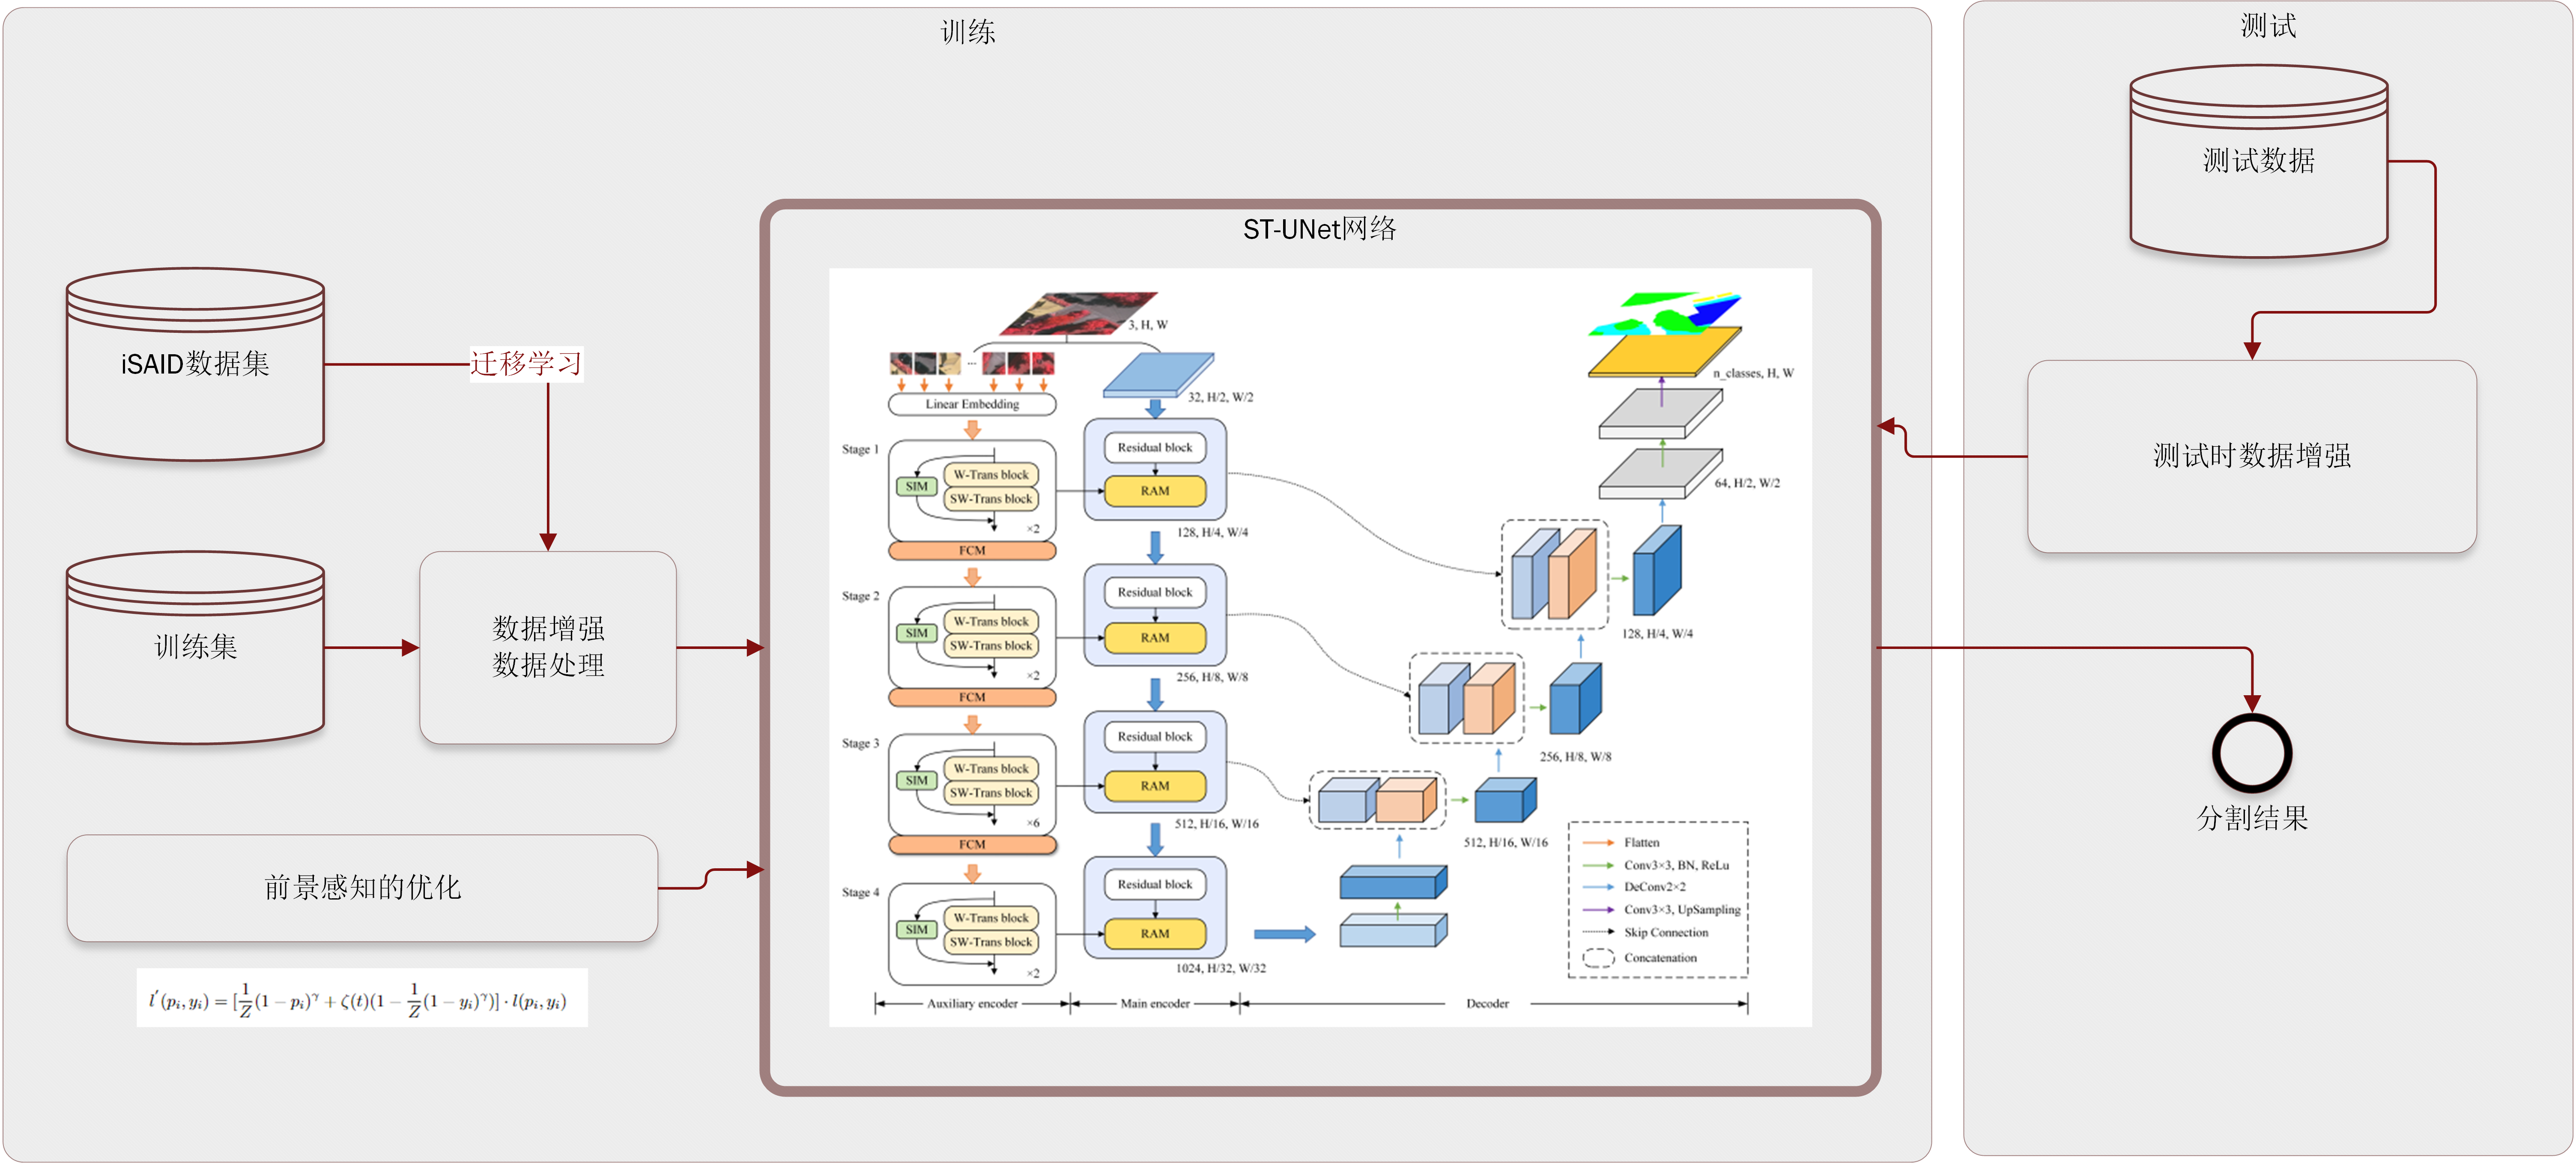
\includegraphics[width=\textwidth]{flowchart.png}
    \centering
    \caption{整体设计}
    \label{fig:fulldesign}
\end{figure}

图~\ref{fig:fulldesign}是我们的整体设计示意图。我们计划使用通过混合CNN和Swin-Transformer结构在遥感影像语义分割上取得了良好效果的
\emph{嵌入了Swin Transformer的UNet(ST-UNet)}\cite{stunet}作为网络结构进行调整和训练。
该网络结构融合了Swin-Transformer和有成熟广发应用的CNN结构,可以期望能达到
较好的效果。

为了处理遥感图像分割中样本的不均衡问题,尤其是前景-背景的不均衡问题,我们计划试验使用
FarSeg\cite{farseg}中提出的\emph{前景感知的优化},即使用损失函数\eqref{eqn:newloss}

\begin{equation}
    \label{eqn:newloss}
    l^{'}(p_i,y_i)=[\frac{1}{Z}(1-p_i)^\gamma+\zeta (t)(1-\frac{1}{Z}(1-y_i)^\gamma)]\cdot l(p_i,y_i)
\end{equation}

通过以背景中的困难部分作为权重较高的部分,可以是网络集中在前景和背景中的困难样本中,从而实现均衡优化。

Transformer主干网络的模型通常相对于CNN为主干网络的模型难以训练。为了解决这个问题,我们将应用\emph{迁移学习}的方法。
考虑到题目给定的数据集尺寸相对较小,我们首先在更大更完全的遥感影像数据集中预训练该网络,然后再在题目
给定的数据集中进行训练。这是提高准确性的有效方法。我们计划采用iSAID数据集\cite{isaid},该数据集提供了2806张遥感影像,来自
有多种传感器和多分辨率的平台,图象大小从$800\times800$到$4000\times13000$不等。为了使得该数据集
和题目给定的数据集尽可能接近,我们将会对iSAID数据集进行进一步处理,裁切成$256\times256$的分块。

在数据处理方面,我们将对遥感影像进行\emph{数据增强},包括随机裁剪、亮度,对比度和饱和度的调整
加入噪点与随机模糊等。这些影像变换可以模拟遥感图像采集中常见的图像缺陷。这些缺陷可能干扰识别,通过
对训练集进行数据增强,可以降低这些负面因素对网络训练的影响。

在模型实际应用的过程中,我们将会应用\emph{测试时增强}的方法,在测试时通过数据增强产生额外的推理结果
在此基础上进行投票可以获得更好的性能表现。


\chapter{整体设计}

\section{遥感图像分割任务与ST-UNet}
遥感影响的物体分割是一种语义分割任务。这种任务面对大规模的变化、大规模的类内背景差异和较大的类外背景差异。
以及前景-背景不平衡的问题。一般的语义分割常常更加关注自然场景中的尺度变化,而没有充分地考虑到其他的问题\cite{farseg}。
并且常见的CNN作为主干网络的模型由于卷积运算的局部性,难以对网络的全局特征进行直接获取。

Swin Transformer在实践中展现出了极为强大的全局建模能力。而UNet是一种常用、表现优秀的的语义分割框架。因此将Swin Transformer嵌入传统的基于CNN的UNet
中,可以得到ST-UNet这一融合的遥感图像语义分割的框架\cite{stunet},它具有Swin-Transformer
和CNN平行工作的\emph{双Encoder}架构。一方面,ST-UNet使用空间交互模块(Spatial Interation Module, STM)通过Swin Transformer编码像素级
的相关性来提高特征的代表能力,尤其是\emph{受到遮蔽的物体}。另一方面,该模型通过一个特征压缩模块(Feature Compression Module, FPM)来减少
详细信息的丢失,并在补丁标记下采样时浓缩更多的小规模的特征,这些小尺度的特征可以提高地面小尺度物体的分割精度。

最后,作为以上两个编码器的桥梁,该网路通过一个关系聚合模块(Relation Aggregation Module, RAM)来聚合两个编码器的特征,将Swin-Transformer获得的全局相关关系
层级化地集成到CNN中。这种方式对在真实世界数据集中的识别起到了极为显著的提高\cite{stunet}。

在该方案中,我们采用该网络的原因主要有如下两点

\begin{itemize}
    \item Transformer框架在计算机视觉领域有良好的前景
    \item ST-UNet表现出了较好的性能
\end{itemize}


\section{前景感知的优化}
前景感知的优化是\cite{farseg}中提出了重要优化之一。前景与背景不均衡的问题常常导致在训练过程中背景主导了梯度,
但是只有北京的困难部分队训练后期的优化有价值,而这些样本相对稀少。这是该优化提出的动力。它的核心是将损失函数换成
\eqref{eqn:newloss2},借此将网络集中在前景和背景的困难样本上。

\begin{equation}
    \label{eqn:newloss2}
    l^{'}(p_i,y_i)=[\frac{1}{Z}(1-p_i)^\gamma+\zeta (t)(1-\frac{1}{Z}(1-y_i)^\gamma)]\cdot l(p_i,y_i)
\end{equation}

其中$p_i$是预测的概率,$y_i$代表第$i$像素的Ground truth。$Z$是一个归一化常数,该常数保证$\sum l(p_i,y_i)=\frac{1}{Z}\sum(1-p_i)^\gamma l(p_i,y_i)$。
$l(p_i,y_i)$是一个交叉熵损失函数。$\zeta(t)$是一个单调递减的退火函数,其取值范围在$[0,1]$之间。有线性、多项式、余弦三种选择,如图~\ref{fig:annel_func},
每种选择有各自的超参数可供控制和调整。

\begin{figure}[htbp]
    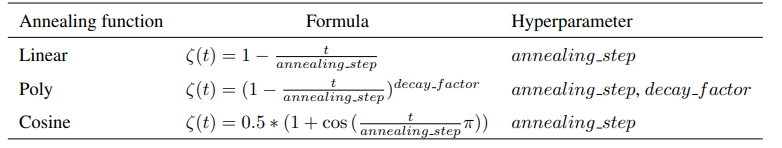
\includegraphics[width=\textwidth]{annealing_funcs.png}
    \centering
    \caption{退火函数}
    \label{fig:annel_func}
\end{figure}

虽然该优化和主干网络ST-UNet并不来源于同一个工作,但是该优化对遥感图像分割任务中有显著影响的不均衡问题提出了
解决方案,该解决方案与主干网络独立,具有一定的普适性。因此将该优化加入ST-UNet中以测试其性能并作为一种
可能的优化候选是合理的,一定程度上也是必要的。

\section{迁移学习}
\blindtext

\section{数据增强}
\blindtext


\part{实现方法}

\chapter{模型实现}

\section{主干网络和前景感知的优化}
\blindtext

\section{迁移学习和数据增强}
\blindtext

\chapter{训练与测试}

\section{训练方法}
尽管Transformer在图象上的应用具有较强的竞争力,但是与成熟的卷积神经网络相比,训练技巧还并不成熟\cite{howtotrain},
并且由于参数量的区别,Transformer训练通常较难。因此,本方案对ST-UNet的训练提出以下的预案

\subsubsection{迁移学习}

本方案反复强调了迁移学习的重要性。这是因为\cite{howtotrain}中提到,就大多数实际目的而言,迁移预先训练的模型不仅成本效益较高,
而且会带来更好的结果。对于类似题目所给的这样数据量相对同邻域常用数据集较小的数据集而言,几乎不可能
通过从零开始训练使其达到接近迁移模型的精度。而对于足够大的数据集,从零开始达到与迁移模型相似的精度
则需要多花超过2个数量级的时间。

\section{消融试验}

消融试验是一种常用的方法,为了检验采取多项改进时每一项改进都对效果的提高具有正向贡献,
需要对各项改进单独出现、成组出现的情况进行测试。由于本方案为了有效地进行遥感图像语义分割进行了多项措施,
为了检验各项措施,我们将进行消融试验,并依照试验结果进行评估,对措施进行重新调整,试验计划如表~\ref{tbl:ablexpr}。

\begin{table}[htbp]
    \centering
    \caption{消融试验计划}
    \label{tbl:ablexpr}
    \renewcommand\arraystretch{1.5}
    \begin{tabular}{ccc|c}
        \toprule
        \hline
        前景感知的优化 & 额外数据集的迁移学习 & 数据增强 & mIOU\\
        \hline
        $\checkmark$ & \ & \ & 待测 \\
        \ & $\checkmark$ & \ & 待测  \\
        \ & \ & $\checkmark$ & 待测  \\
        $\checkmark$ & $\checkmark$ & \ & 待测  \\
        $\checkmark$ & \ & $\checkmark$ & 待测  \\
        \ & $\checkmark$ & $\checkmark$ & 待测  \\
        $\checkmark$ & $\checkmark$ & $\checkmark$ & 待测 \\
        \hline
        \bottomrule
    \end{tabular}
\end{table}

我们期望在消融试验中得到性能参数逐次增高的效果。如果某项措施的效果不能达到预期的效果,
我们会考虑
\begin{itemize}
    \item 对该项措施进行重新调整;
    \item 移除该项措施
\end{itemize}
然后重新进行测试并评估效果。

\part*{参考文献}
\addcontentsline{toc}{part}{参考文献}

\bibliographystyle{unsrt}
\bibliography{reference}

\appendix
\part*{附录}
\addcontentsline{toc}{part}{附录}

\section*{Section within the appendix}
\blindtext

\end{document}